Não existe, no momento, nenhuma infraestrutura no local para as
realização dos testes, sendo necessário a implementação da infraestrutura civil,
elétrica e de suporte para os testes.

Primeiramente, o objetivo principal dos testes consistia em realizar um processo
de pintura automática, simulando o processo de metalização e com forte apelo
visual para o cliente. Entretanto, como será exposto a seguir, a infraestrutura
necessária para o processo é extensa e os paramêtros realmente testados não são
explícitos.

\subsection{Pintura}

Sistema de Pintura: para a utilização de um sistema de pintura é necessária a utilização de sistemas de: 
compressão de ar, purificação de ar, compressão de tinta, isolamento e exaustão.

Compressão de ar: O ar necessário para o sistema deve ser limpo e seco. Para isso é necessário utilizar 
um compressor de diafragma, no qual não existe contato do pistão com o ar a ser comprido ou um filtro de 
óleo. A umidade também afeta o sistema e é necessário a utilização de filtros desumidificadores e condensadores 
de água. Entretanto para o propósito em questão, acredito que apenas um compressor de diafragma seria suficiente, 
pois não há necessidade de uma pintura de qualidade.

Compressão de tinta: As pistolas de tinta podem ser dividas, basicamente, em dois grandes grupos: pistolas a 
gravidade e pistolas automáticas. A primeira classe possui um recipiente onde é
armazenada a tinta e é acoplada à pistola. Essa característica restringe o
movimento do conjunto, forçando que o efetuador fique orientado sempre com o
recipiente na vertical. Essa restrição adicional é desnecessaŕia para o nosso teste e, por isso, desclassifica esse tipo de pistola como um possível dispositivo para a realização do mesmo. A segunda 
categoria utiliza, além da alimentação de ar comprimido, uma alimentação de tinta proveniente de um 
tanque de pressão de tinta.

Outro fator importante é o isolamento da "cabine de pintura" e a correta exaustão do ar do particulado em 
suspensão. A pistola de tinta pulveriza a tinta em direção à peça a ser pintada e parte dessa tinta fica 
em suspensão no ambiente, impregnando as paredes e objetos próximos. A presença humana nesse ambiente requer 
máscaras de respiração e proteção para olhos e roupas, e qualquer equipamento
eletrônico próximo seria danificado, incluindo computadores e o próprio
controlador e manipulador. Sendo assim, é necessário o isolmanento da
área onde será realizada a pintura e proteção do manipulador. Outro ponto a ser
considerado  é a realização de exaustão, filtragem e
descarte corretos da tinta, para que não se danifique nenhuma estrutura
adjacente ao local de testes (LEAD e prédios vizinhos).

A área útil de metalização realizada pela pistola é de 3mm e as pistolas automáticas são para pinturas de grandes 
superfícies, não sendo possível uma cobertura tão precisa. Portanto, o propósito
do teste é prejudicado e a pintura serviria apenas como um indicativo visual,
não representando a real trajetória do efetuador e nem a real cobertura
realizada.

Portanto, não acredito que o investimento de capital, tempo e mão de obra para a construção de uma infraestrutura 
de pintura para o teste de viabilidade técnica para o projeto EMMA 1 justifique os benefícios alcançados por esse 
tipo de procedimento. Outro fator limitante é o espaço ocupado por todos os equipamentos em comparação com o 
espaço disponível no momento, como será apresentado a seguir. Também será apresentado alternativas de testes 
possíveis para ser realizados com o espaço e tempo disponíveis, que consigam avaliar os requisitos mínimos para 
a viabilidade técnica do processo de metalização realizado pelo sistema proposto.  

\subsection{Configuração mínima}

A partir do espaço disponível, foi realizado um esboço de uma configuração
mínima de testes. Como pode ser observado na figura \ref{fig::planta}, a
acomodação dos itens necessários se dá de maneira apertada. A
configuração mínima necessária foi considerada como: uma pá em escala 1:1, uma
seção do trilho primário servindo apenas como ponto de apoio e pivoteamento,
trilho secundário de 2,75m, manipulador MH12 e seu controlador DX200.

\begin{figure}[h!]
\centering
	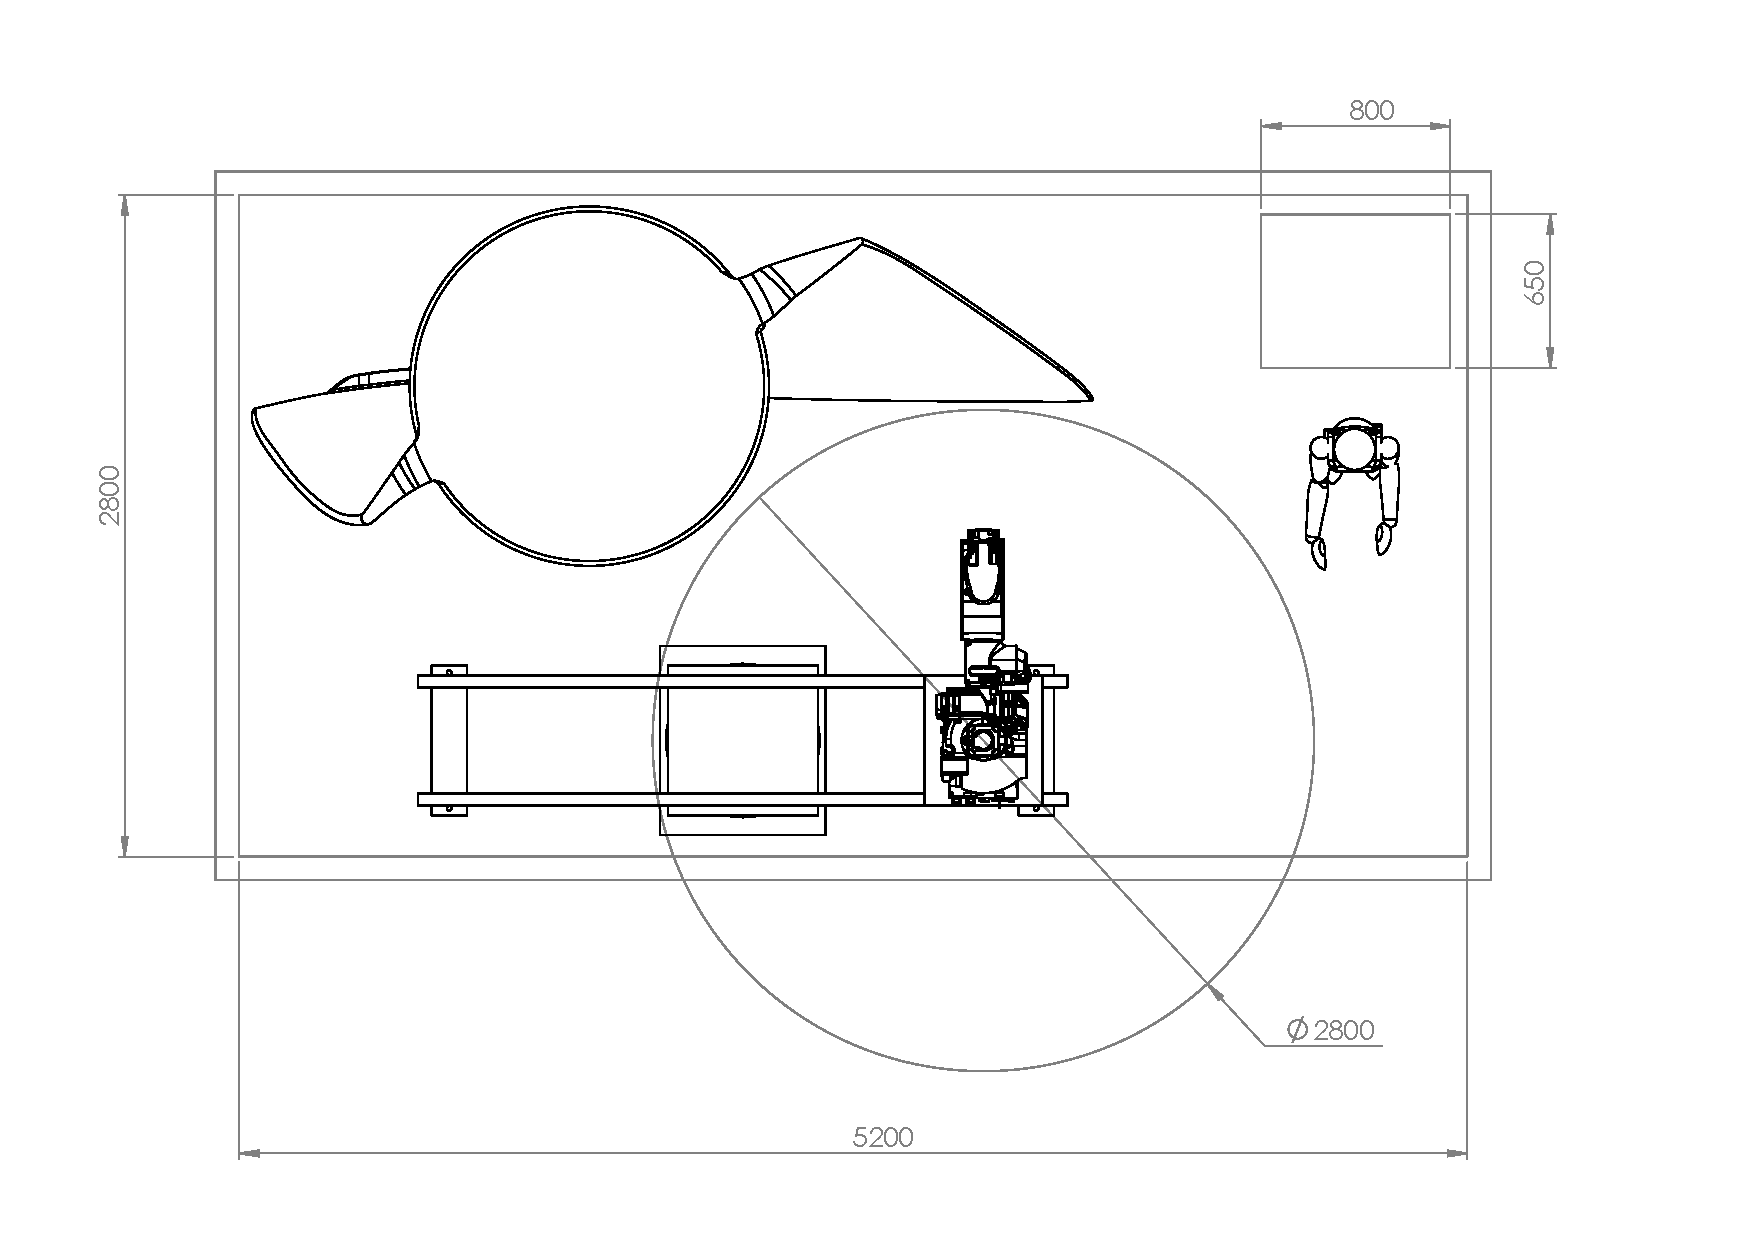
\includegraphics[width=0.9\columnwidth]{figs/espaco/Montagem_Base_LEAD}
	\caption{Espaço disponível e possível disposição dos elementos necessários
	para os testes.}
	\label{fig::planta}
\end{figure}


Pode-se observar que o robô não tem seu espaço de trabalho totalmente livre. As
paredes ficam dentro de seu alcance, representando um perigo estrutural
para o ambiente,  existindo apenas uma posição para a sua base que possibilita
um espaço livre no semi circulo frontal do robô, essa seria a unica área que teríamos para realizar testes 
antes de simular o coating da pá. Esse cenário não é o ideal, uma vez que até o teste final, 
é necessário um espaço para livre movimentação sem risco de colisões. 

\subsection{Demanda Elétrica}

DX200 - 3-phase, 240/480/575 VAC at 50/60 Hz
MH12 -	1.5 kVA

\subsection{Base do manipulador MH12}
O manipulador deve possuir uma base padrão instalada no ambiente de testes, para
que seja possível a realização de testes, modificações e reparos na base e
trilho propostos. 
A princípio, não é necessário que a base suporte o robô em
movimento, entrentanto caso haja espaço suficiente, essa possibilidade é
interessante para os testes relacionados apenas ao manipulador sem que haja
influência da base projetada.


\subsection{Movimentação de equipamentos pesados}
O manipulador MH12 deverá ser movimentado constantemente na área de testes e tem
peso de $130kg$, por isso julga-se necessário a implementação de um sistema de
talha e carro trole. O carro trole pode se movimentar em uma viga I pertencente
a própria estrutura de sustentação do ambiente de testes, ou permanente fixada
no mesmo. A estrutura de movimentação deve permitir o transporte entre do
manipulador a partir de sua base até o local de testes de cobertura, para
acoplamento à estrutura mecânica.


\subsection{Bancada de trabalho}
É necessário um espaço para trabalho para pelo menos 1 pessoa.
Primeiramente foi idealizado a utilização da área ocupada pelo controlador DX200
e a construção de uma bancada de apoio. 
Portanto, afim de se poupar espaço, o
controlador ficaria embaixo da bancada e a pessoa trabalhando nos testes usaria
o computador em pé.

 \subsection{Suporte da pá 1:1}
 O suporte da maquete em escala 1:1 da pá deve, idealmente, o giro da pá em
 torno de seu próprio eixo vertical e horizontal. 
 O movimento no eixo vertical possibilita o teste de cobertura em ambos os lados
 da pá, caso contrário é necessário retirar a pá do suporte e realizar o giro.
 É importante ressaltar que dependendo do tamanho do galpão em que o teste seja
 realizado, não será possível a movimentação da pá, sendo necessário a retirada
 da pá de dentro do ambiente para manobra.
 
 \subsection{Fluxo de equipamentos}
- Dimensões dos equipamentos que etram e saem (dimensionamento da porta);

